\section{Versuchsaufbau/-durchführung}

\subsection{Versuchsaufbau}
Der grundlegende Aufbau ist in der Abbildung \ref{fig: aufbau} illustriert.
\begin{figure}[!h]
  \centering
  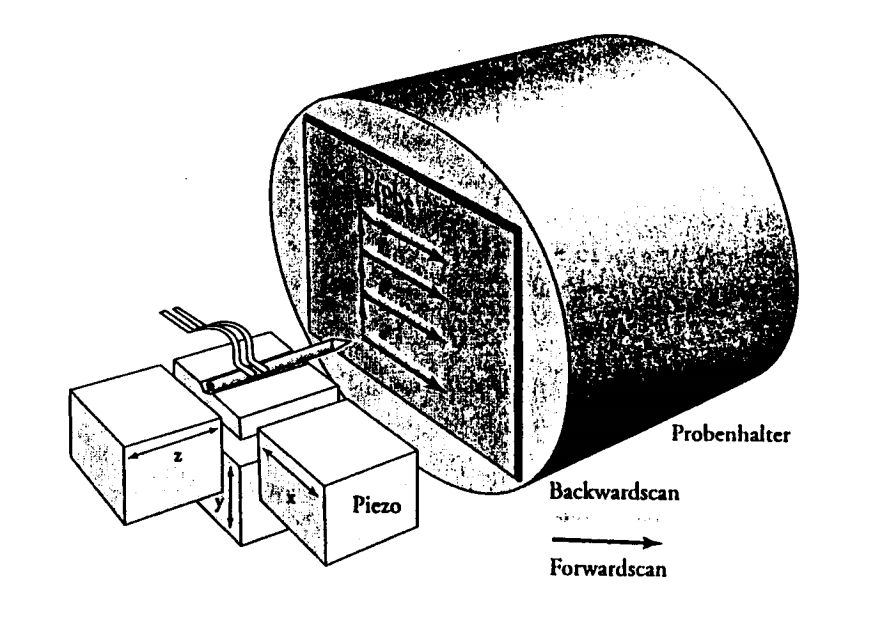
\includegraphics[width=0.6\textwidth]{./pics/aufbau.png}
  \caption{Grundlegender Aufbau eines Rastertunnelmikroskops \cite{anleitung_frankfurt}.}
  \label{fig: aufbau}
\end{figure}
In der Abbildung ist die Spitzenhalterung und
der Probenhalter mit Probe zu sehen. Die Apparatur wird mittels Computersoftware gesteuert.
Die in dem Schema zu erkennenden Piezokeramiken werden
verwendet, um die Spitze filigran zu bewegen. %filigran

Beim Abrastern der Probe gibt es zwei Methoden die atomare Struktur zu erfassen.
Zum einen ist es möglich den Abstand zwischen Probe und Spitze konstant zu halten (CHM, constant height method)
und die Veränderung des Tunnelstroms zu messen. %vielleicht noch fachabkürzung ergänzen (hier)
Jedoch bietet dieses Verfahren die Gefahr, dass die Spitze die Probe rammt und so unbrauchbar wird.
Umgekehrt ist es möglich, den Tunnelstrom konstant zu lassen und den Abstand zu variieren (CCM, constant current method).
Um die Spitze exakt zu manövrieren wird neben einem Piezokristall ein geeigneter Regelkreis benötigt. %geeigneter
Der Regelkreis stellt eine genaue Ansteuerung des Piezokristalls sicher.
Der verwendete Regelkreis misst den Tunnelstrom und vergleicht ihn mit einem
eingestellten Sollwert. Bei einer Differenz der beiden Werte wird die Höhe des Piezoelements
entsprechend angepasst. Die Anpassgeschwindigkeit lässt sich über zwei Parameter
einstellen. Zum einen den \emph{integralen Anteil}, dieser beeinflusst im Wesentlich die %Wesentlichen
Geschwindigkeit mit der auf Abweichungen reagiert wird. Zum anderen kann der %Abweichungen
\emph{propotionale Anteil} verändert werden,
er regelt, wie stark auf eine Abweichung reagiert wird.
Die Werte vom integralen und proportionalen Anteil hängen von der Art der
Oberflächenuntersuchung ab.

\subsection{Versuchsdurchführung}

Für eine genaue Messung wird eine einatomige Spitze benötigt.
Hergestellt wird die Spitze aus \ce{PtIr}-Draht (Platin-Iridium)
mit Hilfe einer Pinzette, einer Zange und eines Seitenschneiders.
Bevor mit den Materialien eine Spitze erstellt werden kann, müssen sie mit Aceton und Propanol gereinigt werden. %kann,
Damit die Spitze besonders fein wird, werden die Werkzeuge wie in Abbildung \ref{fig: zange_schneider}
dargestellt positioniert.
\begin{figure}[!h]
  \centering
  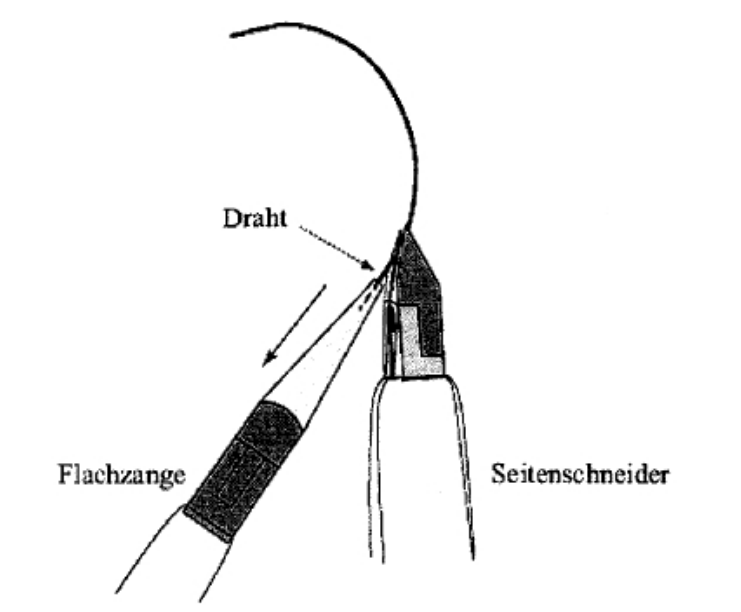
\includegraphics[width=0.6\textwidth]{./pics/herstellung_spitze.png}
  \caption{Positionierung des Seitenschneiders und der Zange am Draht. \cite{anleitung_frankfurt}.}
  \label{fig: zange_schneider}
\end{figure}
Anschließend werden Zange und Schneider in entgegensetzte Richtung gezogen.
Dabei ist von essentieller Bedeutung, dass der Draht wirklich auseinander gezogen wird und
nicht geschnitten.

Nachdem eine Spitze gerissen wurde, wird der Probenhalter in das Rastertunnelmikroskop eingesetzt.
Anschließend wird der Probenhalter mit der Probe in das RTM eingeführt.
Nun muss die Probe nah genug an die Spitze herangeführt werden, dies wird zu Beginn
manuell gemacht. Die Probe wird manuell so nah an die Spitze herangeführt, bis sich
die Spitze und ihr Spiegelbild beinah berühren. Die Software für das automatische
Heranführen überprüft regelmäßig, ob ein Tunnelstrom detektiert werden kann oder nicht. %komma zu viel
Wird zum Beispiel kein Tunnelstrom gemessen so wird die Probe, von der Software %komma zu viel
näher an die Spitze gefahren $\left(I\propto \frac{1}{d}\exp{(-d)}\right) $.
Deshalb ist es wichtig, bevor der automatische
Modus verwendet wird, eine Spannung an der Spitze anzulegen $\left(I\propto U\right)$. Mit Hilfe einer
Statusleuchte kann kontrolliert werden, ob ein Tunnelstrom detektiert wird. Außerdem zeigt die Leuchte
ob die Spitze die Probe berührt hat.
Sobald die Software fertig mit der Justage ist, beginnt automatisch die Messung.
Bei der Messung wird unterschieden, ob die Spitze von rechts nach links (backward) oder von links nach rechts (forward) %begriffe foreward und backward einführen
die Probe abrastert. Mit der Unterscheidung soll die Auswirkung von Hysterese Effekte überprüfbar werden. %wird damit nicht verringert aber ist überprüfbar
Auf jeder, der in der Skizze \ref{fig: aufbau} dargestellten, Linie wird eine vorher eingestellte
Anzahl an Messungen durchgeführt.

In dem Versuch werden eine HOPG- und Goldprobe vermessen.
Bei der HOPG-Probe sollen die Gittervektoren der atomaren Struktur
experimentell bestimmt werden.
Bei der Goldprobe wird mit Hilfe des Höhenprofils der Goldoberfläche implizit
die Gitterkonstante des fcc-Gitters in $[111]$-Richtung ermittelt.
